\section{Data Mapping}

\subsection{{\tt nodes} Directive}

The {\tt nodes} directive declares a {\it node array}, which is an
array-like arrangement of nodes in a node set. A node array can be
multi-dimensional.

%\subsubsection{One-dimensional Node Set}

\begin{XCexample}
#pragma xmp nodes p[4]
\end{XCexample}

\begin{XFexample}
!$xmp nodes p(4)
\end{XFexample}

The nodes directive declares a one-dimensional node array \|p| that
includes four nodes. In XMP/C, it is zero-based and consists
of \|p[0]|, \|p[1]|, \|p[2]|, and \|p[3]|. In XMP/Fortran, it is
one-based and consists of \|p(1)|, \|p(2)|, \|p(3)|, and \|p(4)|.

%\subsubsection{Multi-dimensional Node Set}

\begin{XCexample}
#pragma xmp nodes p[2][3]
\end{XCexample}

\begin{XFexample}
!$xmp nodes p(3,2)
\end{XFexample}

The \|nodes| directive declares two-dimensional node array \|p| that
includes six nodes. In XMP/C, it consists of \|p[0][0]|,
\|p[0][1]|, \|p[0][2]|, \|p[1][0]|, \|p[1][1]|, and \|p[1][2]|. In
XMP/Fortran, it consists of \|p(1,1)|, \|p(2,1)|, \|p(3,1)|,
\|p(1,2)|, \|p(2,2)|, and \|p(3,2)|.

\begin{mynote}
  The ordering of the elements in a node array follows that of a normal
  array in the base language, C or Fortran. 
\end{mynote}

%\subsubsection{Dynamic Node Set}

\begin{XCexample}
#pragma xmp nodes p[*]
\end{XCexample}

\begin{XFexample}
!$xmp nodes p(*)
\end{XFexample}

An asterisk can be specified as the size in the \|nodes| directive to declare a
{\it dynamic} node array. In the above code, one-dimensional dynamic
node array \|p| is declared with an asterisk as the size. The actual
size of a dynamic node array is determined at runtime to fit the size of
the current executing node set.
%
For example, when
the programmer runs the sample code with three nodes, the node array
\|p| includes three nodes.

They can also declare multi-dimensional dynamic node arrays with an
asterisk.

\begin{XCexample}
#pragma xmp nodes p[*][3]
\end{XCexample}

\begin{XFexample}
!$xmp nodes p(3,*)
\end{XFexample}

When the programmer runs the sample code with 12 nodes, the node array \|p|
has a shape of 4x3, in C, or 3x4, in Fortran.

\begin{mynote}
  The user can put an asterisk only in the last dimension, in
  XMP/Fortran, or the first dimension, in XMP/C of the node array.
\end{mynote}

\begin{myhint}
  The dynamic node array may interfere with compiler optimizations. In
  general, programs with static ones achieve better performance.
\end{myhint}

%\subsubsection{Partial Node Set}

The programmer can declare a node subarray derived from an existing node
array. Node subarrays can be used, for example, to optimize inter-node
communication by reducing the number of nodes participating in the
communication.

\begin{XCexample}
#pragma xmp nodes p[16]
#pragma xmp nodes q[8]=p[0:8]
#pragma xmp nodes r[4][2]=p[8:8]
\end{XCexample}

\begin{XFexample}
!$xmp nodes p(16)
!$xmp nodes q(8)=p(1:8)
!$xmp nodes r(2,4)=p(9:16)
\end{XFexample}

In line 1, a node array \|p| including 16 nodes is declared. In line 2, a
node subarray \|q| corresponding to the first half of \|p| is declared. In line 3, a
two-dimensional node subarray \|r| corresponding to the latter half of \|p| is declared.

The programmer can declare a n-dimensional node subarray derived from a m-dimensional one.

\begin{XCexample}
#pragma xmp nodes p[4][2]
#pragma xmp nodes row[4]=p[:][*]
#pragma xmp nodes col[2]=p[*][:]
\end{XCexample}

\begin{XFexample}
!$xmp nodes p(2,4)
!$xmp nodes row(4)=p(*,:)
!$xmp nodes col(2)=p(:,*)
\end{XFexample}

In line 1, a two-dimensional node array \|p| including 4x2 nodes is
declared. In line 2, a node subarray \|row| derived from a single row of
\|p| is declared. In line 3, a node subarray \|col| derived from a
single column of \|p| is declared.

A colon represents a triplet which indicate all possible indices in the
dimension.
%
An asterisk indicate the index of the current executing node in the
dimension.
%
For example, \|col[2]| corresponds to \|p[0][0:2]| on nodes \|p[0][0]| and
\|p[0][1]|, and to \|p[1][0:2]| on nodes \|p[1][0]| and \|p[1][1]| in
XMP/C. Similarly, \|col(2)| corresponds to \|p(1:2,1)| on nodes
\|p(1,1)| and \|p(2,1)|, and to \|p(1:2,2)| on nodes \|p(1,2)| \|p(2,2)|
in XMP/Fortran.

\begin{figure}
  \centering
  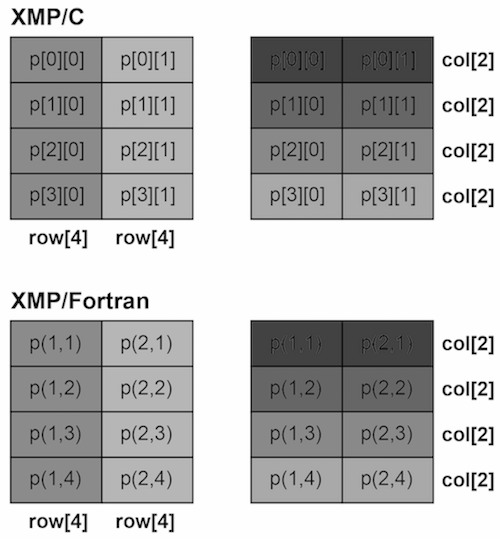
\includegraphics{figs/row_col.png}
  \caption{Node subarrays.}
  \label{fig:partial}
\end{figure}

In XMP/C, \|row[0]| corresponds to \|p[0][0]| and \|p[0][1]| on
\|p[:][0]| and \|p[:][1]|, respectively; 
%
\|col[0]| corresponds to \|p[0][0]|, \|p[1][0]|, \|p[2][0]|, and \|p[3][0]|
on \|p[0][:]|, \|p[1][:]|, \|p[2][:]|, \|p[3][:]|, respectively.
%
In XMP/Fortran, \|row(1)| corresponds to \|p(1,1)| and \|p(2,1)| on
\|p(1,:)| and \|p(2,:)|, respectively;
%
\|col(1)| corresponds to \|p(1,1)|, \|p(1,2)|, \|p(1,3)|, and \|p(1,4)|
on \|p(:,1)|, \|p(:,2)|, \|p(:,3)|, \|p(:,4)|, respectively.

\begin{mynote}
  The semantics of an asterisk in a node reference is different from
  that in a declaraion.
\end{mynote}


\subsection{{\tt template} Directive}

The \|template| directive declares a {\it template}, which is a virtual
array that is used as a ``template'' of parallelization in the programs
and to be distributed onto a node array.
%  Templates are virtual arrays which used for data and work 
% mapping. They can have multi-dimensional shapes.

%\subsubsection{One-dimensional Template}

\begin{XCexample}
#pragma xmp template t[10]
\end{XCexample}

\begin{XFexample}
!$xmp template t(10)
\end{XFexample}

This \|template| directive declares a one-dimensional template \|t|
having ten elements.
%
Templates are indexed in the similar manner to
arrays in the base languages. For the above examples, the template \|t|
is indexed from zero to nine (i.e. \|t[0]| $\cdots$ \|t[9]|), in XMP/C,
or one to ten (i.e. \|t(1)| $\cdots$ \|t(10)|), in XMP/Fortran.

\begin{myhint}
% In general, the user declare templates which has the same
% size with the target data array.
  In many cases, a template should be declared to have the same shape as
  your target array.
\end{myhint}

% In XMP/Fortran, the start index of the template can be given by an
% arbitrary number to match the starting array index in the base
% language.

% \begin{XFexample}
% !$xmp template t(-5:4)
% \end{XFexample}

% The template directive declares 1-dimensional template t starting from t(-5) to t(4).

% \begin{mynote}
% In XMP/C, templates should start from 0 since array indices
% start from 0 in the C language.
% \end{mynote}

%\subsubsection{Multi-dimensional Template}

\begin{XCexample}
#pragma xmp template t[10][20]
\end{XCexample}

\begin{XFexample}
!$xmp template t(20,10)
\end{XFexample}

The \|template| directive declares a two-dimensional template \|t| that
has 10x20 elements. In XMP/C, \|t| is indexed from t[0][0] to t[9][19],
and,  in XMP/Fortran, from \|t(1,1)| to \|t(20,10)|.

%\subsubsection{Dynamic Template}

\begin{XCexample}
#pragma xmp template t[:]
\end{XCexample}

\begin{XFexample}
!$xmp template t(:)
\end{XFexample}

In the above examples, a colon instead of an integer is specified as the
size to declare a one-dimensional dynamic template \|t|. The colon
indicates that the size of the template is not fixed and to be
fixed at runtime by the \|template_fix| construct (Sec. \ref{184243_1Nov19}).


\subsection{{\tt distribute} Directive}

The \|distribute| directive specifies a distribution of the target
template.
%
Either of {\it block}, {\it cyclic}, {\it block-cyclic}, or {\it gblock}
(i.e. uneven block) can be specified to distribute a dimension of a template.


\subsubsection{Block Distribution}

\begin{XCexample}
#pragma xmp distribute t[block] onto p
\end{XCexample}

\begin{XFexample}
!$xmp distribute t(block) onto p
\end{XFexample}

The target template \|t| is divided into contiguous blocks and
distributed among nodes in the node array \|p|.
%
% When the size of the template is $N$ and the
% number of nodes is $K$, the size of each block will be $ceil(N/K)$.
Let's suppose that the size of the template is $N$ and the
number of nodes is $K$. If $N$ is divisible by $K$, a block of size $N/K$
are assigned to each node; otherwise, a block of size
$ceil(N/K)$ is assigned to each of $N/ceil(N/K)$ nodes, a block of size
$mod(N,K)$ to one node, and no block to $(K-N/ceil(N/K)-1)$ nodes. 
%
The block distribution is useful for regular computations such as a
stencil one.

\begin{mynote}
  The function $ceil(x)$ returns a minimum integer value greater than
  $x$, and $mod(x,y)$ returns $x$ modulo $y$.
\end{mynote}

\begin{XCexample}
#pragma xmp nodes p[3]
#pragma xmp template t[22]
#pragma xmp distribute t[block] onto p
\end{XCexample}

\begin{XFexample}
!$xmp nodes p(3)
!$xmp template t(22)
!$xmp distribute t(block) onto p
\end{XFexample}

\begin{figure}
  \centering
  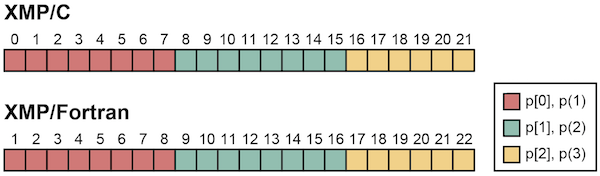
\includegraphics{figs/block.png}
  \caption{Block distribution.}
\end{figure}

Since $ceil(22/3)$ is 8, eight elements are allocated on each of \|p[0]|
and p[1], and the remaining six elements are allocated on \|p[2]|.

% The user can explicitly specify the block size.
% In that case, the remaining elements are allocated on the last node.

% \begin{XCexample}
% #pragma xmp nodes p[3]
% #pragma xmp template t[22]
% #pragma xmp distribute t[block(7)] onto p
% \end{XCexample}

% \begin{XFexample}
% !$xmp nodes p(3)
% !$xmp template t(22)
% !$xmp distribute t(block(7)) onto p
% \end{XFexample}

% \begin{figure}
%   \centering
%   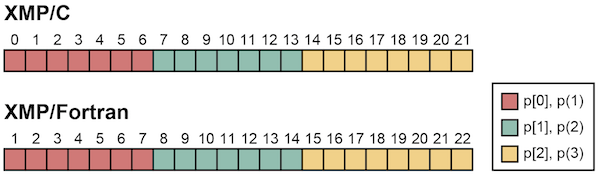
\includegraphics{figs/block2.png}
% \end{figure}

% Seven elements will be allocated on the p[0] and p[1], as specified in
% the directive. And then remaining 8 elements will be allocated on the
% last node p[2].


\subsubsection{Cyclic Distribution}

\begin{XCexample}
#pragma xmp distribute t[cyclic] onto p
\end{XCexample}

\begin{XFexample}
!$xmp distribute t(cyclic) onto p
\end{XFexample}

The target template \|t| is divided into chunks of size one and
distributed among nodes in the node array \|p| in a round-robin manner.
%
The cyclic distribution is usefull for the case where the load on each
element of the template is not balanced.
%suitable for computation with an irregular
%load%balance of data and computation.

\begin{XCexample}
#pragma xmp nodes p[3]
#pragma xmp template t[22]
#pragma xmp distribute t[cyclic] onto p
\end{XCexample}

\begin{XFexample}
!$xmp nodes p(3)
!$xmp template t(22)
!$xmp distribute t(cyclic) onto p
\end{XFexample}

\begin{figure}
  \centering
  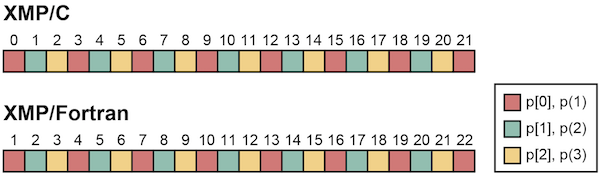
\includegraphics{figs/cyclic.png}
  \caption{Cyclic distribution.}
\end{figure}


\subsubsection{Block-cyclic Distribution}

\begin{XCexample}
#pragma xmp distribute t[cyclic(w)] onto p
\end{XCexample}

\begin{XFexample}
!$xmp distribute t(cyclic(w)) onto p
\end{XFexample}

The target template \|t| is divided into chunks of size \|w| and distributed
among nodes in the node array \|p| in a round-robin manner.
%
The block-cyclic distribution is usefull for the case where the load on
each element of the template is not balanced but the locality of the
elements is required.

% Block-cyclic distribution is
% suitable for computation which has an irregular load balance and
% references to neighborhood elements.

\begin{XCexample}
#pragma xmp nodes p[3]
#pragma xmp template t[22]
#pragma xmp distribute t[cyclic(3)] onto p
\end{XCexample}

\begin{XFexample}
!$xmp nodes p(3)
!$xmp template t(22)
!$xmp distribute t(cyclic(3)) onto p
\end{XFexample}

\begin{figure}
  \centering
  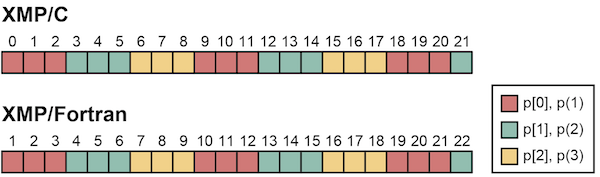
\includegraphics{figs/block-cyclic.png}
  \caption{Block-cyclic distribution.}
\end{figure}


\subsubsection{Gblock Distribution}

\begin{XCexample}
#pragma xmp distribute t[gblock(W)] onto p
\end{XCexample}

\begin{XFexample}
!$xmp distribute t(gblock(W)) onto p
\end{XFexample}

The target template \|t| is divided into contiguous blocks of size \|W[0]|,
\|W[1]|, $\cdots$, in XMP/C, or \|W(1)|, \|W(2)|, $\cdots$, in
XMP/Fortran, and distributed among nodes in the node array \|p|.
%
The array \|W| is called a mapping array.
%
The programmer can specify irregular (uneven) block distribution with
the gblock format.
%a special type of data distribution explicitly by using
%mapping arrays (e.g. distribution of triangular matrix).

\begin{XCexample}
#pragma xmp nodes p[3]
#pragma xmp template t[22]
int W[3] = {6, 11, 5};
#pragma xmp distribute t[gblock(W)] onto p
\end{XCexample}

\begin{XFexample}
!$xmp nodes p(3)
!$xmp template t(22)
integer, parameter :: W(3) = (/6,11,5/)
!$xmp distribute t(gblock(W)) onto p
\end{XFexample}

\begin{figure}
  \centering
  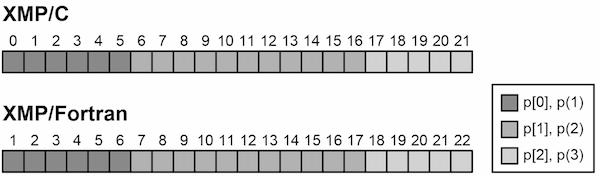
\includegraphics{figs/gblock.png}
  \caption{Gblock distribution.}
\end{figure}

The programmer can specify an asterisk instead of a mapping array in the 
gblock distribution to defer fixing the actual distribution.
%
In such a case, the actual distribution will be fixed at runtime by 
using {\tt template\_fix} construct.


\subsubsection{Distribution of Multi-dimensional Templates}

The programmer can distribute a multi-dimensional template onto
a node array.

\begin{XCexample}
#pragma xmp nodes p[2][2]
#pragma xmp template t[10][10]
#pragma xmp distribute t[block][block] onto p
\end{XCexample}

\begin{XFexample}
!$xmp nodes p(2,2)
!$xmp template t(10,10)
!$xmp distribute t(block,block) onto p
\end{XFexample}

The \|distribute| directive declares the distribution of a two-dimensional
template \|t| onto a two-dimensional node array \|p|. Each dimension of the
template is divided in a block manner and each of the rectangular
regtion is assigned to a node.

\begin{figure}
  \centering
  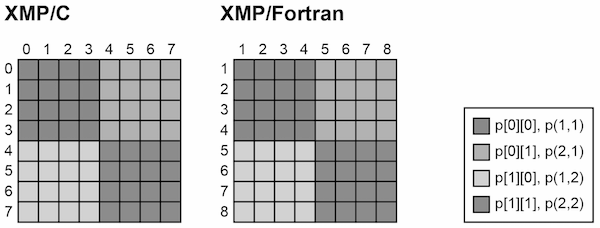
\includegraphics{figs/multi.png}
  \caption{Example of multi-dimensional distribution (1).}
\end{figure}

The programmer can specify a different distribution format in each of
the dimension of a template.

\begin{XCexample}
#pragma xmp nodes p[2][2]
#pragma xmp template t[10][10]
#pragma xmp distribute t[block][cyclic] onto p
\end{XCexample}

\begin{XFexample}
!$xmp nodes p(2,2)
!$xmp template t(10,10)
!$xmp distribute t(cyclic,block) onto p
\end{XFexample}

\begin{figure}
  \centering
  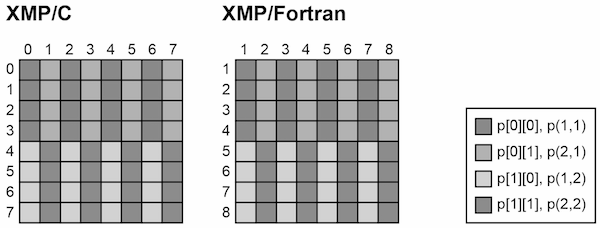
\includegraphics{figs/multi2.png}
  \caption{Example of multi-dimensional distribution (2).}
\end{figure}

When an asterisk is specified in a \|distribute| directive as
a distribution format, the target dimension is ``non-distributed.'' In
the following example, the first dimension is distributed in a
block manner and the second dimension is non-distributed.

\begin{XCexample}
#pragma xmp nodes p[4]
#pragma xmp template t[10][10]
#pragma xmp distribute t[block][*] onto p
\end{XCexample}

\begin{XFexample}
!$xmp nodes p(4)
!$xmp template t(10,10)
!$xmp distribute t(*,block) onto p
\end{XFexample}

\begin{figure}
  \centering
  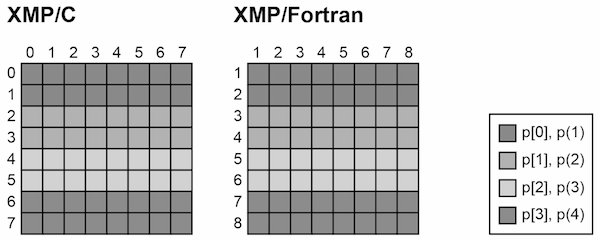
\includegraphics{figs/multi3.png}
  \caption{Example of multi-dimensional distribution (3).}
\end{figure}


\subsection{{\tt align} Directive}

% The {\tt align} directive performs data mapping and distributes data
% among nodes by using a distributed template. The {\tt align} directive
% must follow the definition of the target template.

The \|align| directive specifies that an array is to be mapped in the
same way as a specified template. In other words, an \|align| directive
defines the correspondece of elements between an array and a template,
and each of the array element is allocated on the node where the
corresponding template element is allocated.
% As a result of this directive, an array is ``distributed'' onto nodes.

%\subsubsection{Normal Alignment}

\begin{XCexample}
#pragma xmp nodes p[4]
#pragma xmp template t[8]
#pragma xmp distribute t[block] onto p
int a[8];
#pragma xmp align a[i] with t[i]
\end{XCexample}

\begin{XFexample}
!$xmp nodes p(4)
!$xmp template t(8)
!$xmp distribute t(block) onto p
integer :: a(8)
!$xmp align a(i) with t(i)
\end{XFexample}

The array \|a| is decomposed and laid out so that each element
\|a(i)| is colocated with the corresponding template element \|t(i)|.

% The {\tt align} directive aligns the owner node of a[i] with t(i), a
% distributed template. As a result, array a is distributed among the node
% set p.

\begin{figure}
  \centering
  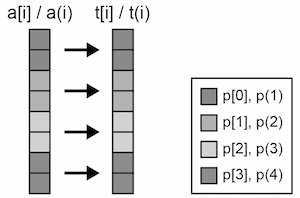
\includegraphics{figs/1dim.png}
  \caption{Example of array alignment (1).}
\end{figure}

The \|align| directive can also be used for multi-dimensional arrays.

\begin{XCexample}
#pragma xmp nodes p[2][2]
#pragma xmp template t[8][8]
#pragma xmp distribute t[block][block] onto p
int a[8][8];
#pragma xmp align a[i][j] with t[i][j]
\end{XCexample}

\begin{XFexample}
!$xmp nodes p(2,2)
!$xmp template t(8,8)
!$xmp distribute t(block,block) onto p
integer :: a(8,8)
!$xmp align a(j,i) with t(j,i)
\end{XFexample}

\begin{figure}
  \centering
  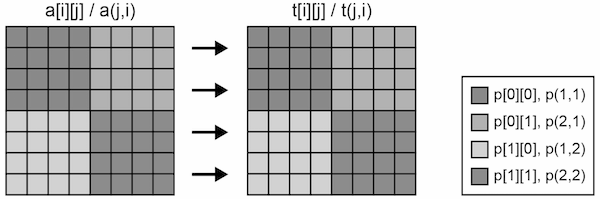
\includegraphics{figs/multi-dim.png}
  \caption{Example of array alignment (2).}
\end{figure}

%\subsubsection{Special Alignment}

%\paragraph{Collapse}

The programmer can align an $n$-dimensional array with an $m$-dimensional
template for $n > m$.

\begin{XCexample}
#pragma xmp nodes p[4]
#pragma xmp template t[8]
#pragma xmp distribute t[block] onto p
int a[8][8];
#pragma xmp align a[i][*] with t[i]
\end{XCexample}

\begin{XFexample}
!$xmp nodes p(4)
!$xmp template t(8)
!$xmp distribute t(block) onto p
integer :: a(8,8)
!$xmp align a(*,i) with t(i)
\end{XFexample}

When an asterisk is specified as a subscript in a dimension of the
target array in the \|align| directive, the dimension is ``collapsed''
(i.e. not distributed). In the sample program above, the first dimension of the
array {\tt a} is distributed onto the node array \|p| while the second
dimension is collapsed.

\begin{figure}
  \centering
  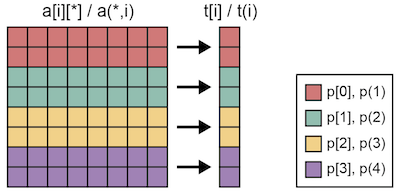
\includegraphics{figs/collapse.png}
  \caption{Example of array alignment (3).}
\end{figure}

In XMP/C, {\tt a[0:2][:]} will be allocated on {\tt p[0]} while, in
XMP/Fortran, \|a(:,1:2)| will be allocated on \|p(1)|.

%\paragraph{Replicate}

The programmer also can align an $n$-dimensional array with an
$m$-dimensional template for $n < m$.

\begin{XCexample}
#pragma xmp nodes p[2][2]
#pragma xmp template t[8][8]
#pragma xmp distribute t[block][block] onto p
int a[8];
#pragma xmp align a[i] with t[i][*]
\end{XCexample}

\begin{XFexample}
!$xmp nodes p(2,2)
!$xmp template t(8,8)
!$xmp distribute t(block,block) onto p
integer :: a(8)
!$xmp align a(i) with t(*,i)
\end{XFexample}

When an asterisk is specified as a subscript in a dimension of the
target template in the \|align| directive, the array will be
``replicated'' along the axis of the dimension.

\begin{figure}
  \centering
  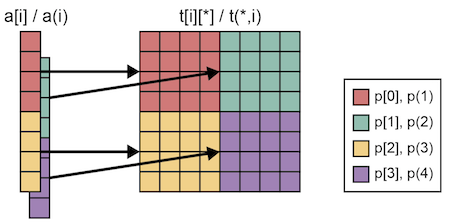
\includegraphics{figs/replicate.png}
  \caption{Example of array alignment (4).}
\end{figure}

In XMP/C, \|a[0:4]| will be replicated and allocated on p[0][0] and
p[0][1] while, in XMP/Fortran, \|a(1:4)| will be allocated on \|p(1,1)|
and \|p(2,1)|.


\subsection{Dynamic Allocation of Distributed Array}

This section explains how distributed (i.e. global) arrays are allocated
at runtime. The basic procedure is common in XMP/C and XMP/Fortran with
a few specific difference.

%\subsubsection{One-dimensional Array}

\begin{XCexample}
#pragma xmp nodes p[4]
#pragma xmp template t[N]
#pragma xmp distribute t[block] onto p
float *a;
#pragma xmp align a[i] with t[i]
  :
a = xmp_malloc(xmp_desc_of(a), N);
\end{XCexample}

In XMP/C, first, declare a pointer of the type of the target array; 
%
second, align it as if it were an array;
%
finally, allocate memory for it with the {\tt xmp\_malloc()}
function. {\tt xmp\_desc\_of()} is an 
intrinsic/builtin function that returns the descriptor of the XMP object
(i.e. nodes, templates, or global arrays) specified by the argument.

\begin{XFexample}
!$xmp nodes p(4)
!$xmp template t(N)
!$xmp distribute t(block) onto p
real, allocatable :: a(:)
!$xmp align a(i) with t(i)

allocate(a(N))
\end{XFexample}

In XMP/Fortran, first, declare an allocatable array; second, align it;
finally, allocate memory for it with the \|allocate| statement.

%\subsubsection{Multi-dimensional Array}

For multi-dimensional arrays, the procedure is the same as that for 
one-dimensional ones, as follows:

\begin{XCexample}
#pragma xmp nodes p[2][2]
#pragma xmp template t[N1][N2]
#pragma xmp distribute t[block][block] onto p
float (*a)[N2];
#pragma xmp align a[i][j] with t[i][j]
  :
a = (float (*)[N2])xmp_malloc(xmp_desc_of(a), N1, N2);
\end{XCexample}

\begin{XFexample}
!$xmp nodes p(2,2)
!$xmp template t(N2,N1)
!$xmp distribute t(block,block) onto p
real, allocatable :: a(:,:)
!$xmp align a(j,i) with t(j,i)
  :
allocate(a(N2,N1))
\end{XFexample}

\begin{mynote}
  If the size of the template is not fixed until runtime, the programmer
  have to fixe it at runtime with the \|template_fix| construct.
\end{mynote}


\subsection{{\tt template\_fix} Construct}
\label{184243_1Nov19}

The \|template_fix| construct fixes the shape and/or the distribution of
an unfixed template. 
%It is also used when a distributed array is allocated at runtime.

\begin{XCexample}
#pragma xmp nodes p[4]
#pragma xmp template t[:]
#pragma xmp distribute t[block] onto p
double *a;
#pragma xmp align a[i] with t[i]

int n = 100;
#pragma xmp template_fix t[n]
a = xmp_malloc(xmp_desc_of(a), n);
\end{XCexample}

\begin{XFexample}
!$xmp nodes p(4)
!$xmp template t(:)
!$xmp distribute t(block) onto p
real, allocatable :: a(:)
integer :: n
!$xmp align a(i) with t(i)

n = 100
!$xmp template_fix t(n)
allocate(a(n))
\end{XFexample}

In the above sample code, 
%
first, a template \|t| whose size is unfixed (``\|:|'') is declared;
%
second, a pointer \|a|, in XMP/C, or an allocatable array \|a|, in
XMP/Fortran, is aligned with the template;
%
third, the size of the template is fixed with a \|template_fix|
construct;
%
finally, the pointer or the allocatable array is allocated with the
\|xmp_malloc()| builtin function in XMP/C or the \|allocate| statement
in XMP/Fortran, respectively.

\begin{mynote}
The {\tt template\_fix} constructs can be applied to a template only once.
\end{mynote}

This construct can also be used to fix a mapping array of a template
that is distributed in ``\|gblock(*)|`` at declaration.

\begin{XCexample}
#pragma xmp nodes p[4]
#pragma xmp template t[:]
#pragma xmp distribute t[gblock(*)] onto p
double *a;
#pragma xmp align a[i] with t[i]

int n = 100;
int m[] = {40,30,20,10};

#pragma xmp template_fix[gblock(m)] t[n]
a = xmp_malloc(xmp_desc_of(a), n);
\end{XCexample}

\begin{XFexample}
!$xmp nodes p(4)
!$xmp template t(:)
!$xmp distribute t(gblock) onto p
real, allocatable :: a(:)
integer :: n, m(4)
!$xmp align a(i) with t(i)

n = 100
m(:) = (/40,30,20,10/)
!$xmp template_fix(gblock(m)) t(n)
allocate(a(n))
\end{XFexample}
